\chapter{The Polar Front as a major biogeographic boundary in the Southern Ocean} 
\label{ch:polarfront}

Sections of this chapter have been previously published in \bibentry{Wilkins:2012td}.

\section{Summary}

\section{Introduction}


\section{Methods}
\subsection{Sampling and metagenomic sequencing}

Sampling\footnote{Sampling was performed by Jeffrey M. Hoffman and Jeffrey B. Mcquaid} was conducted on board the RSV \emph{Aurora Australis} during cruise V3 \ac{CEAMARC/CASO} from 13 December 2007 -- 26 January 2008. 
This cruise occupied the SR3 latitudinal transect from Hobart, Australia (44\textdegree{} S) to the Mertz Glacier, Antarctica (67\textdegree{} S) within a longitudinal range of 140--150\textdegree{} E.
Nineteen samples (16 surface, 3 deep) were obtained along almost the entire latitudinal range \figref{fig:samplemap}.

% the sample map
\begin{figure}[!ht]
  \centering
  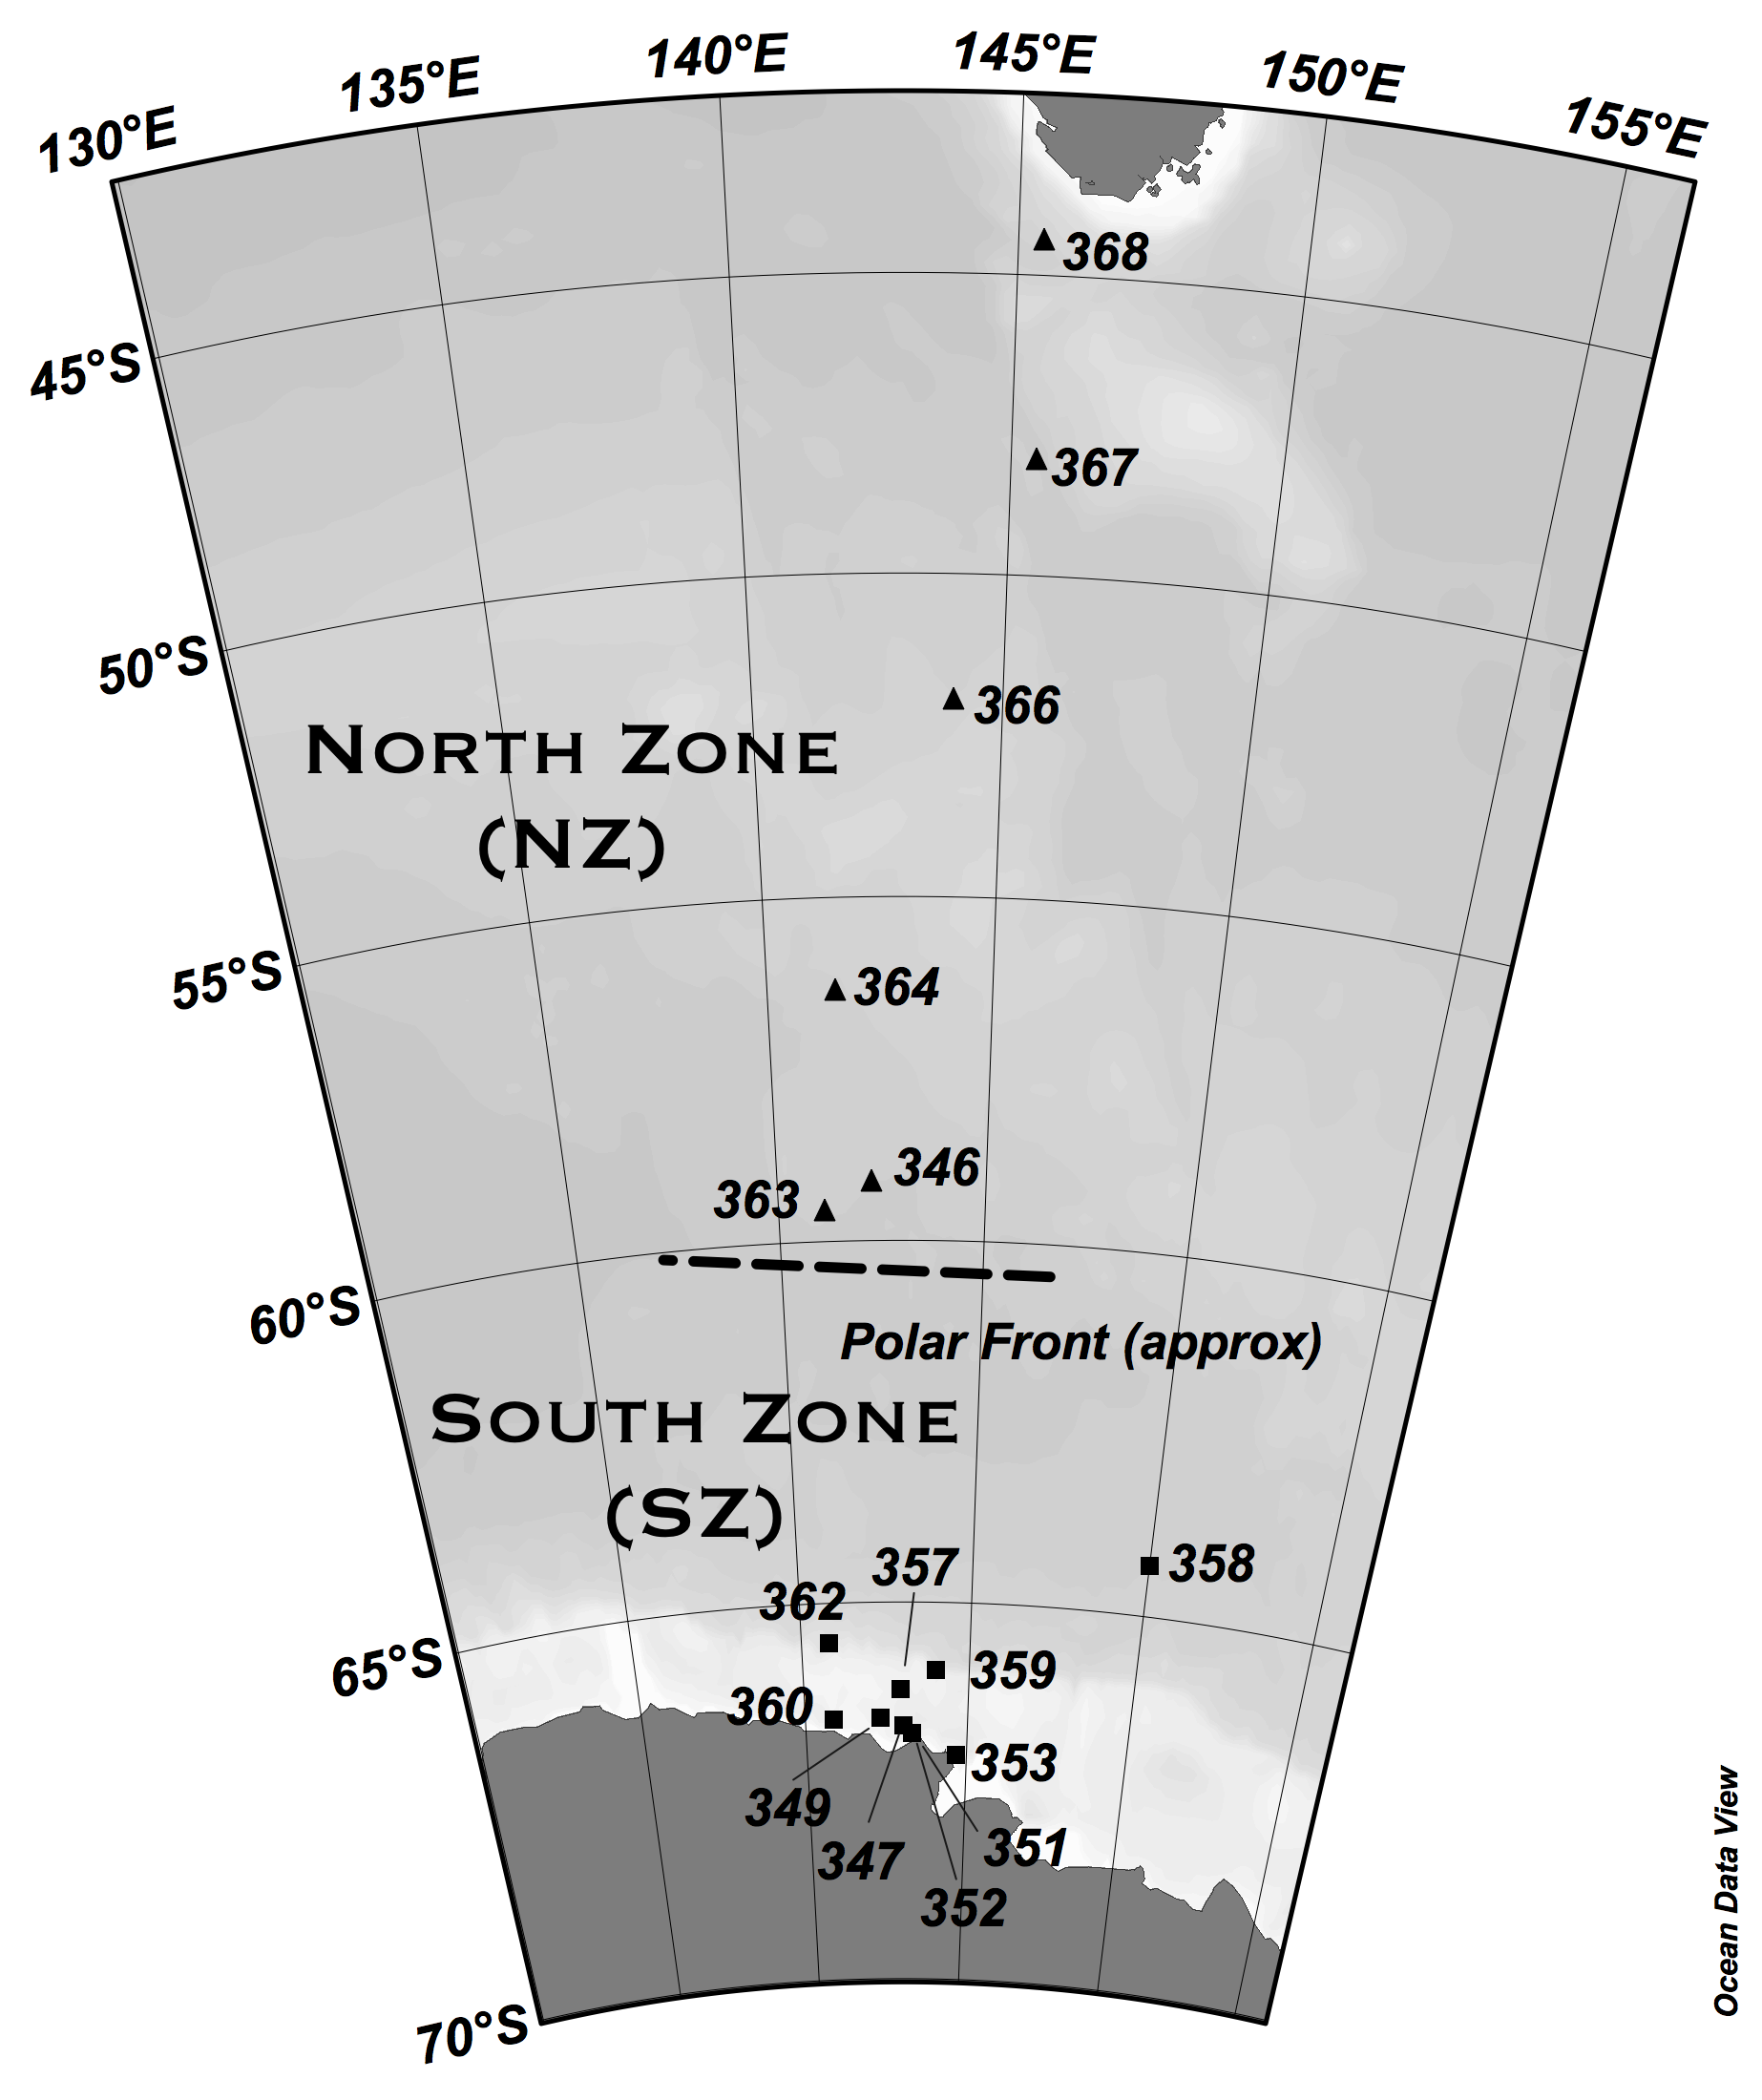
\includegraphics[width=\textwidth]{../polarfront/samplemap.png}
  \caption[Map showing sites of seawater samples used in the Polar Front study]{Sites of seawater samples used in this study. 
  Squares indicate surface samples from the North Zone; crosses samples from the South Zone. 
  The dashed line represents the Polar Front.}
  \label{fig:samplemap}
\end{figure}


A range of data were recorded by integrated instruments on the RSV \emph{Aurora Australis} including location, water column depth, water temperature, salinity, fluorescence and meterological data \tabref{tab:samplelist}.
These data were used to locate the \ac{PFZ} based on a surface temperature gradient of $\sim$ 1.35 \textdegree{}C across a distance of 45--65 km, placing the \ac{PF} at approximately $-59.70$\textdegree{} of latitude, consistant with previous descriptions \cite{Moore:1999to,Sokolov:2002tc}.
Samples were accordingly grouped into ``North'' and ``South'' zones, while the three deep samples composed a ``Deep'' zone \tabref{tab:samplelist}.
The \ac{NZ} represents waters from the Subtropical, Subantarctic and \ac{PFZ} regions, while the \ac{SZ} represents the \ac{AZ}.

\begin{sidewaystable}
\sffamily
\caption[Details of samples used in Polar Front study]{\sffamily{}Sampling time, location and physicochemical properties of samples used in this study.
All data were retrieved from underway instruments aboard the RSV \textit{Aurora Australis}.}
\label{tab:samplelist}
\smallskip
\begin{tabularx}{\textheight}{lllXXXXXXXX}
\toprule
\textbf{Sample} & \textbf{Zone} & \textbf{Date} & \textbf{Latitude} & \textbf{Longitude} & \textbf{Water \linebreak Column \linebreak Depth (m)} & \textbf{Sample Depth (m)} & \textbf{Temperature (\textdegree{}C)} & \textbf{Salinity (PSU)} & \textbf{Fluorescence \linebreak (\textmu{}gL\textsuperscript{\textminus{}1})} & \textbf{Volume \linebreak filtered (L)}\\
\midrule

346 & North & 20/12/2007 & \textminus{}59.31 & 142.59 & 4294 & 2 & 2.9 & 33.75 & 0.3 & 500\\
347 & South & 23/12/2007 & \textminus{}66.02 & 142.74 & 450 & 2 & 0.6 & 34.20 & 4.0 & 250\\
349 & South & 27/12/2007 & \textminus{}66.57 & 142.32 & 370 & 1.5 & \textminus{}1.3 & 34.40 & 2.3 & 250\\
351 & South & 28/12/2007 & \textminus{}66.56 & 143.43 & 823 & 1.5 & \textminus{}0.6 & 34.30 & 1.3 & 500\\
352 & South & 29/12/2007 & \textminus{}66.77 & 143.32 & 164 & 2.5 & \textminus{}0.8 & 34.30 & 3.1 & 500\\
353 & South & 30/12/2007 & \textminus{}67.05 & 144.68 & 180 & 2 & \textminus{}1.8 & 34.40 & 0.3 & 500\\
357 & South & 05/01/2008 & \textminus{}66.17 & 143.02 & 580 & 2 & \textminus{}0.4 & 34.15 & 2.5 & 500\\
358 & South & 09/01/2008 & \textminus{}64.30 & 150.03 & 3550 & 2 & 0 & 33.55 & 0.5 & 500\\
359 & South & 12/01/2008 & \textminus{}66.19 & 143.53 & 540 & 2 & \textminus{}0.2 & 34.21 & 2.5 & 500\\
360 & South & 13/01/2008 & \textminus{}66.58 & 141.02 & 316 & 2 & \textminus{}0.7 & 34.04 & 6.2 & 500\\
362 & South & 19/01/2008 & \textminus{}65.54 & 140.83 & 1064 & 2 & 0.7 & 32.20 & 0.5 & 500\\
363 & North & 22/01/2008 & \textminus{}60.00 & 141.31 & 4473 & 2 & 3.3 & 33.77 & 0.1 & 500\\
364 & North & 23/01/2008 & \textminus{}56.70 & 141.88 & 3693 & 2 & 4 & 33.70 & 0.5 & 500\\
366 & North & 24/01/2008 & \textminus{}52.02 & 144.14 & 3180 & 2 & 7.6 & 33.84 & 0.3 & 500\\
367 & North & 25/01/2008 & \textminus{}48.25 & 145.90 & 3490 & 2 & 11 & 34.43 & 0.2 & 500\\
368 & North & 26/01/2008 & \textminus{}44.72 & 145.78 & 3201 & 2 & 14.8 & 34.96 & 1.3 & 560\\

\bottomrule
\end{tabularx}
\end{sidewaystable}


At each station, $\sim$ 250--560 L of seawater was pumped from $\sim$ 1.5--2.5 m below the sea surface into drums stored at ambient temperature on deck. 
In the case of deep samples, $\sim$ 225--230 L of seawater was collected from Niskin bottles attached to a \ac{CTD} (SeaBird, Bellevue, USA).
Seawater samples were prefiltered through a 20 \micron plankton net, then filtrate was captured on sequential 3.0 \micron 0.8 \micron and 0.1 \micron 293 mm polyethersulfone membrane filters (Port Washington, USA), and immediately stored at $-20$ $^\circ$C \cite{Rusch:2007ez,Ng:2010cd}.

DNA extraction\footnote{DNA extraction was performed by Cynthia Andrews-Pfannkoch and others at the J. Craig Venter Institute} was performed at the J. Craig Venter Institute (Rockville, USA) as described in \citet{Rusch:2007ez}.
Pyrosequencing was performed on a GS20 FLX Titanium instrument (Roche, Branford, USA) also at the J. Craig Venter Institute as described in \citet{Lauro:2010jna}.
Duplicate reads and reads with many pyrosequencing errors were removed as described in \citet{Lauro:2010jna}.

\subsection{Phylogenetic analysis of metagenomic data}

\subsubsection{\softwarename{blast} comparison to RefSeq database}

A subset of the RefSeq microbial (bacterial and archaeal) genome database (release 41, retrieved May 31 2012 from \url{ftp://ftp.ncbi.nih.gov/refseq/release/}) was prepared by excluding sequences with the words ``shotgun'', ``contig'', ``partial'', ``end'' or ``part'' in their headers \cite{Angly:2009ip}.
Because this database was not expected to contain representative genomes for every species present, \acp{OTU} in this study are defined by the best species match to this database, and may for example represent congeners.

The metagenomic reads from each sample were compared against this database using \softwarename{tblastx}, with default parameters except for: E-value threshold $1.0\times{}10^{-3}$, cost to open gap 11, cost to extend gap 1, masking of query sequence by \softwarename{SEG} masking with lookup table only.

\subsubsection{Identification of minimal species sets with \softwarename{minspec}}

A computational method to minimise false \ac{OTU} identifications and increase the accuracy of \ac{OTU} abundance estimates (\softwarename{minspec}) was developed and implemented in \softwarename{perl}.
Following the approach of \citet{Ye:2009bl} to the parsimonious reconstruction of biochemical pathways (\softwarename{MinPath}), \softwarename{minspec} computes the smallest set of OTUs sufficient to explain a set of observed high-quality hits against RefSeq (or any other sequence database).
The minimal set computation is framed as a linear programming problem and solved with the \ac{GLPK} tool \ac{GLPSOL} (Free Software Foundation, Boston).
This approach eliminates many of the spurious \ac{OTU} identifications which result from reads with strong identity to more than one \ac{OTU}. 
The ``minimal species set'' is liable to exclude some low-abundance \acp{OTU}, but gives more faithful abundance estimates and eliminates many false positives.

To validate this approach and estimate error rates, an assemblage of hypothetical taxa was simulated with varying degrees of overlapping genomic identity and a logarithmic rank-abundance curve. 
A simulated metagenomic sampling and \softwarename{blast} search was performed on this set, and the results processed with \softwarename{minspec}.
The outputs of all \softwarename{tblastx} searches against RefSeq were processed by \softwarename{minspec}, and hits not belonging to the minimal sets were removed.

\subsubsection{\ac{OTU} abundances and variance between zones}

The relative \ac{OTU} abundances for each sample were determined using the \softwarename{perl} script \ac{GAAS} \cite{Angly:2009ip}.
Briefly, \ac{GAAS} estimates the relative abundance of \acp{OTU} from the number and quality of BLAST hits to each species, taking into account differences in genome size. 
\ac{GAAS} was run with the default settings. 
To normalise for reads which did not yield acceptable hits, the relative abundances for each sample were scaled by that sample's effective \softwarename{blast} hit rate. 
An \ac{OTU} profile was generated for each sample by encoding the scaled relative abundance of each \ac{OTU} from each size fraction as a separate variable.

To test the hypothesis that the oceanic zones harbour significantly different communities, \ac{ANOSIM} with 999 permutations was performed on a standardised, log-transformed Bray-Curtis resemblance matrix of \ac{OTU} profiles with \softwarename{PRIMER 6}.
\ac{SIMPER} analysis was performed with \softwarename{PRIMER 6} to identify the contribution of individual \acp{OTU} to differences between the zones. 
All statistical procedures using \softwarename{PRIMER 6} were performed as described by \citet{Clarke:2001ut}.

\subsection{Functional analysis of metagenomic data}

\subsubsection{\softwarename{blast} comparison to \ac{KEGG} database}

In order to identify functional differences between the zones, the set of metagenomic reads from each sample was compared against the \ac{KEGG} GENES database (retrieved July 2 2010 from \url{ftp://ftp.genome.jp/pub/kegg/genes/fasta/genes.pep}) with \softwarename{blastx}, with default parameters except for: maximum number of database sequence alignments 10; E-value threshold $1.0\times10^{-3}$; gap opening penalty 11; gap extension penalty 1; masking of query sequence by \softwarename{SEG} masking for lookup table only.

\subsubsection{Analysis of functional potential}

Genes identified by \softwarename{blastx} were aggregated to \ac{KEGG} ortholog groups according to the \ac{KEGG} Orthology schema (\url{ftp://ftp.genome.jp/pub/kegg/genes/ko}, retrieved Mar 29 2011), and ortholog group abundances calculated for each sample. 
Following \citet{Coleman:2010jj}, a read was considered a hit to a given ortholog group if the top three hits for that read (or all hits if fewer than three total hits) were to genes from the same ortholog group, and had bit scores \textgreater{} 40. 
If the bit score difference between any two top hits was greater than 30, only the hits above this difference were considered.

Ortholog group counts were then used to calculate the abundance of KEGG modules.
Because many ortholog groups are members of more than one module, the abundance $a_m$ of each module $m$ was calculated as 
\[
a_{m}=\sum_{K=1}^{n}\frac{C_{K}}{M_K}
\]
where $n$ is the number of ortholog groups $K$ belonging to module $m$, $C_{K}$ is the number of hits to ortholog group $K$, and $M_{K}$ is the total number of modules to which $K$ belongs.
To account for differences in sequencing depth between samples, module abundances were scaled to 500,000 reads per sample. 
To test the hypothesis that the \ac{NZ} and \ac{SZ} harbour significantly different functional potential, one-way \ac{ANOSIM} with 999 permutations was performed as above on a standardised, log-transformed Bray-Curtis distance resemblance matrix of the module and ortholog group profiles. 
A functional profile was generated for each sample by summing the scaled abundances of each module from all size fractions, and \ac{SIMPER} performed as above to identify modules which contributed highly to the variation in functional potential between the two zones. 
Modules with a high contribution to variance or otherwise of interest were then linked to taxonomy (``taxonomic decomposition'') by noting the genus of the organism associated with each gene in the \ac{KEGG} GENES database and thus calculating the relative contribution of each genus to each module's abundance. 
This allowed functional contributions to be putatively assigned to genera which were not identified in our taxonomic analysis, as the database included gene sequences for organisms for which a full genome was not available.

\section{Results}

\subsection{Metagenomic sequencing}
6.6 Gbp of 454 sequence data representing picoplankton in the size range 0.1 -- 3.0 \micron was obtained from 16 samples. 
After removal of low-quality reads, 454 sequencing yielded 157,507 -- 597,689 reads per sample (mean 354,399) of lengths ranging from 100 to 606 bp (mean 378).

\subsection{Phylogenetic analysis of metagenomic data}

TODO WORKING ON THIS SECTION

The proportion of reads in each sample which yielded matches to RefSeq ranged from 25\% to 85\% (mean 62\%).

The most abundant \acp{OTU} in each sample are given in \tabreft{tab:topotus} and a full list of \ac{OTU} abundances in the supplementary material \suppfile{PF-all-OTUs.csv}.

\begin{sidewaystable}
\sffamily
\caption[Twenty most abundant \acp{OTU}]{\sffamily{}Relative abundances (as percentages) of the twenty most abundant \acp{OTU} identified in this study, in each zone and size fraction.}
\label{tab:topotus}
\smallskip
\begin{tabularx}{\textheight}{Xlllllllll}
\toprule
OTU & \multicolumn{3}{c}{North} & \multicolumn{3}{c}{South} & \multicolumn{3}{c}{Deep}\\
\cmidrule(r){2-4}
\cmidrule(r){5-7}
\cmidrule(r){8-10}
& 0.1 \micron & 0.8 \micron & 3.0 \micron & 0.1 \micron & 0.8 \micron & 3.0 \micron & 0.1 \micron & 0.8 \micron & 3.0 \micron\\
\midrule

\candidatusfull{Pelagibacter ubique} HTCC1062 & 61.76 & 25.00 & 23.87 & 58.85 & 22.40 & 17.61 & 37.05 & 24.56 & 17.66\\
\speciesfull{Nitrosopumilus maritimus} SCM1 & 0.01996 & 0.01438 & 0.009508 & 1.076 & 1.309 & 1.210 & 19.09 & 9.463 & 17.77\\
\candidatusfull{Ruthia magnifica} str. Cm (\speciesfull{Calyptogena magnifica}) & 0.6699 & 0.6458 & 0.5484 & 2.987 & 2.616 & 1.025 & 3.945 & 4.601 & 2.264\\
\genus{Roseobacter} sp. OCh114 & 0.3125 & 2.932 & 1.588 & 0.4477 & 3.994 & 2.657 & 0.1259 & 1.228 & 0.6792\\
\genus{Synechococcus} sp. CC9902 & 0.1081 & 9.837 & 4.973 & 0.0007484 & 0.004156 & 0.09733 & 0.002846 & 0.01502 & 0.01058\\
\speciesfull{Silicibacter pomeroyi} DSS-3 & 0.2578 & 2.286 & 1.154 & 0.3070 & 2.505 & 1.576 & 0.1224 & 0.9417 & 0.4988\\
\speciesfull{Gramella forsetii} strain KT0803 & 0.2412 & 1.210 & 1.755 & 0.4993 & 2.347 & 1.890 & 0.2078 & 0.6179 & 0.5173\\
\candidatusfull{Vesicomyosocius okutanii} strain HA & 0.4634 & 0.4642 & 0.2078 & 1.970 & 1.807 & 0.2174 & 2.480 & 2.662 & 1.167\\
\speciesfull{Robiginitalea biformata} strain HTCC2501 & 0.2751 & 1.099 & 1.297 & 0.4722 & 1.878 & 1.405 & 0.2265 & 0.6188 & 0.6946\\
\speciesfull{Flavobacterium psychrophilum} strain JIP02/86 & 0.1718 & 0.8409 & 1.224 & 0.4316 & 1.960 & 1.598 & 0.1599 & 0.4744 & 0.6001\\
\genus{Synechococcus} sp. CC9311 & 0.03014 & 4.624 & 4.409 & 0.0007221 & 0.002778 & 0.02764 & 0.001580 & 0.002863 & 0.009241\\
\candidatusfull{Puniceispirillum marinum} IMCC1322 & 0.6444 & 2.077 & 1.267 & 0.3586 & 1.377 & 0.7109 & 0.3425 & 1.062 & 0.5345\\
\genus{Silicibacter} sp. TM1040 & 0.2274 & 1.652 & 0.8738 & 0.2709 & 1.803 & 1.233 & 0.07665 & 0.5890 & 0.2957\\
\genus{Jannaschia} sp. DFL-12 & 0.1776 & 1.378 & 0.7350 & 0.2443 & 1.692 & 0.8009 & 0.07338 & 0.6515 & 0.3078\\
\speciesfull{Zunongwangia profunda} strain SM-A87 & 0.1522 & 0.7487 & 1.059 & 0.2968 & 1.410 & 1.204 & 0.1353 & 0.3478 & 0.4971\\
\genus{Colwellia} sp. 34H & 0.02345 & 0.3636 & 2.736 & 0.05207 & 0.5140 & 1.041 & 0.05137 & 0.4687 & 0.8013\\
\speciesfull{Coraliomargarita akajimensis} strain DSM 45221 & 0.03698 & 0.07573 & 0.1197 & 0.1154 & 1.543 & 1.680 & 0.02614 & 0.3040 & 0.2740\\
\genus{Jannaschia} sp. CCS1 & 0.1173 & 0.9344 & 0.4784 & 0.1711 & 1.230 & 0.8239 & 0.05865 & 0.4462 & 0.2118\\
\speciesfull{Pseudoalteromonas atlantica} strain T6c & 0.01251 & 0.4772 & 1.993 & 0.02270 & 0.4089 & 1.132 & 0.02634 & 0.2143 & 0.7459\\
\speciesfull{Saccharophagus degradans} strain 2-40 & 0.06532 & 0.4325 & 0.5429 & 0.1289 & 1.072 & 0.8663 & 0.07798 & 0.2844 & 0.3165\\
\speciesfull{Flavobacterium johnsoniae} strain UW101 & 0.08822 & 0.4220 & 0.6141 & 0.2034 & 0.9389 & 0.8578 & 0.07545 & 0.2255 & 0.3300\\
\speciesfull{Capnocytophaga ochracea} strain DSM 7271 & 0.1143 & 0.4830 & 0.5399 & 0.2314 & 0.8815 & 0.6814 & 0.08964 & 0.2840 & 0.5043\\
\genus{Marinomonas} sp. MWYL1 & 0.03777 & 0.2529 & 0.3026 & 0.1514 & 1.300 & 0.7006 & 0.07393 & 0.2439 & 0.2155\\
\speciesfull{Cellvibrio japonicus} strain Ueda107 & 0.05884 & 0.3080 & 0.3231 & 0.1155 & 0.9917 & 0.4713 & 0.06774 & 0.2981 & 0.2549\\
\speciesfull{Marinobacter hydrocarbonoclasticus} VT8 & 0.04093 & 0.2889 & 0.3883 & 0.08418 & 0.7195 & 0.3848 & 0.1250 & 0.6667 & 1.066\\
\speciesfull{Pseudoalteromonas haloplanktis} strain TAC125 & 0.01389 & 0.2505 & 0.8896 & 0.03427 & 0.3561 & 0.6530 & 0.1092 & 1.203 & 0.1503\\
\speciesfull{Teredinibacter turnerae} strain T7901 & 0.05665 & 0.3051 & 0.3081 & 0.1138 & 0.9174 & 0.5127 & 0.06558 & 0.2649 & 0.1885\\
\speciesfull{Acinetobacter baumannii} strain SDF & 0.004886 & 0.007187 & 0.4073 & 0.006260 & 0.04218 & 1.459 & 0.004285 & 0.01229 & 0.3155\\

\bottomrule
\end{tabularx}
\end{sidewaystable}



TODO RANK ABUNDANCE \figref{fig:rankabundance}

TODO ADD RANK ABUNDANCE INTO METHODS

% the sample map
\begin{figure}
  \centering
  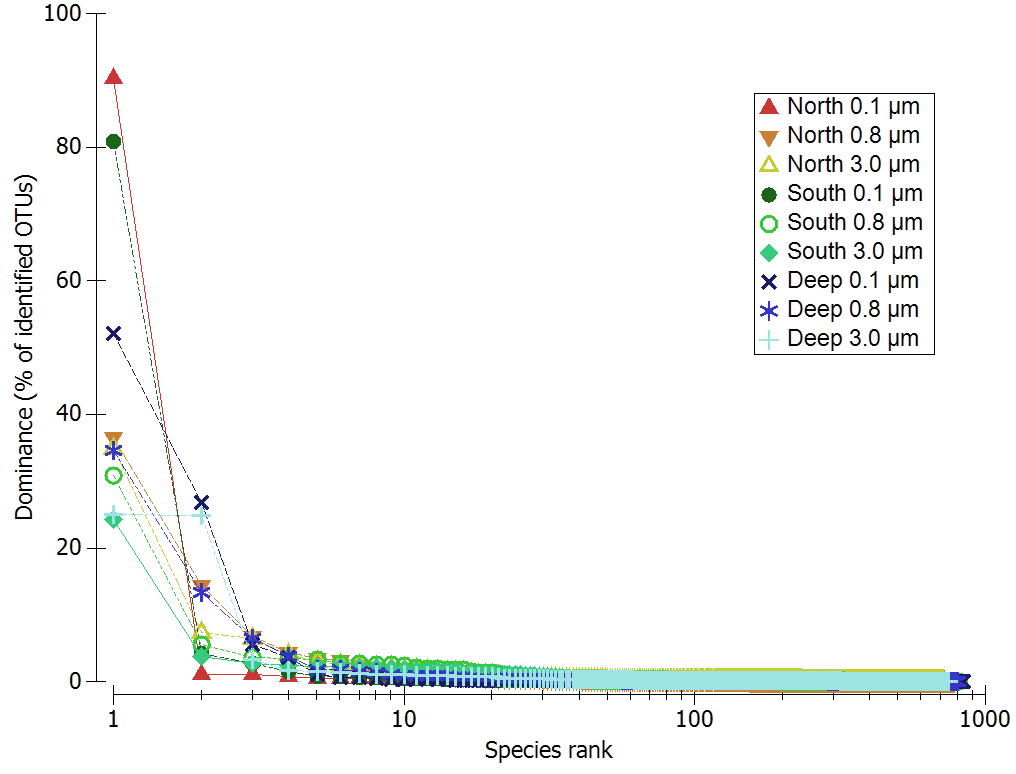
\includegraphics[width=\textwidth]{../polarfront/rankabundance.png}
  \caption[Rank-abundance curves for OTUs in each zone and size fraction]{Rank-abundance curves for OTUs identified in each zone and size fraction. The dominance of a given OTU is its relative abundance as a percentage of all identified OTUs. The x-axis is scaled logarithmically. Generated using \softwarename{PRIMER 6}.}
  \label{fig:rankabundance}
\end{figure}


\ac{ANOSIM} analysis showed that the zones harbor significantly different microbial communities (R = 0.451, p < 0.004). 
\ac{SIMPER} was performed in order to identify the contribution of individual \acp{OTU} to the differences between the \ac{NZ} and \ac{SZ}. 
The \ac{SIMPER} analysis found that no single \ac{OTU} contributed more than 2.9\% of variance TODO REF SIMPER TABLE - SUPP? and 74\% of variance was contributed by \acp{OTU} with a contribution less than 1\%. 
There was also a large difference in the contribution to variance of the three size fractions, with approximately 52\% of all variance contributed by \acp{OTU} from the 3.0 \micron fraction, 37\% by the 0.8 \micron fraction, and 9\% by the 0.1 \micron fraction TODO TABLE (Table S3, supporting information).
Notably, \acp{OTU} within several taxonomic groups that had high contribution to variance covaried in their relative representation in the \ac{NZ} and \ac{SZ}.
For example, Bacteroidetes and GSO-EOSA-1 representatives were on average more abundant in the \ac{SZ}; while \emph{Prochlorococcus} and \emph{Synechococcus} spp., SAR11 and SAR116 were on average more abundant in the \ac{NZ} \figref{taxotreemap}.
Some groups, such as the Alteromonadales, had variable relative representation depending on size fraction.

\begin{figure}[!ht]
  \centering
  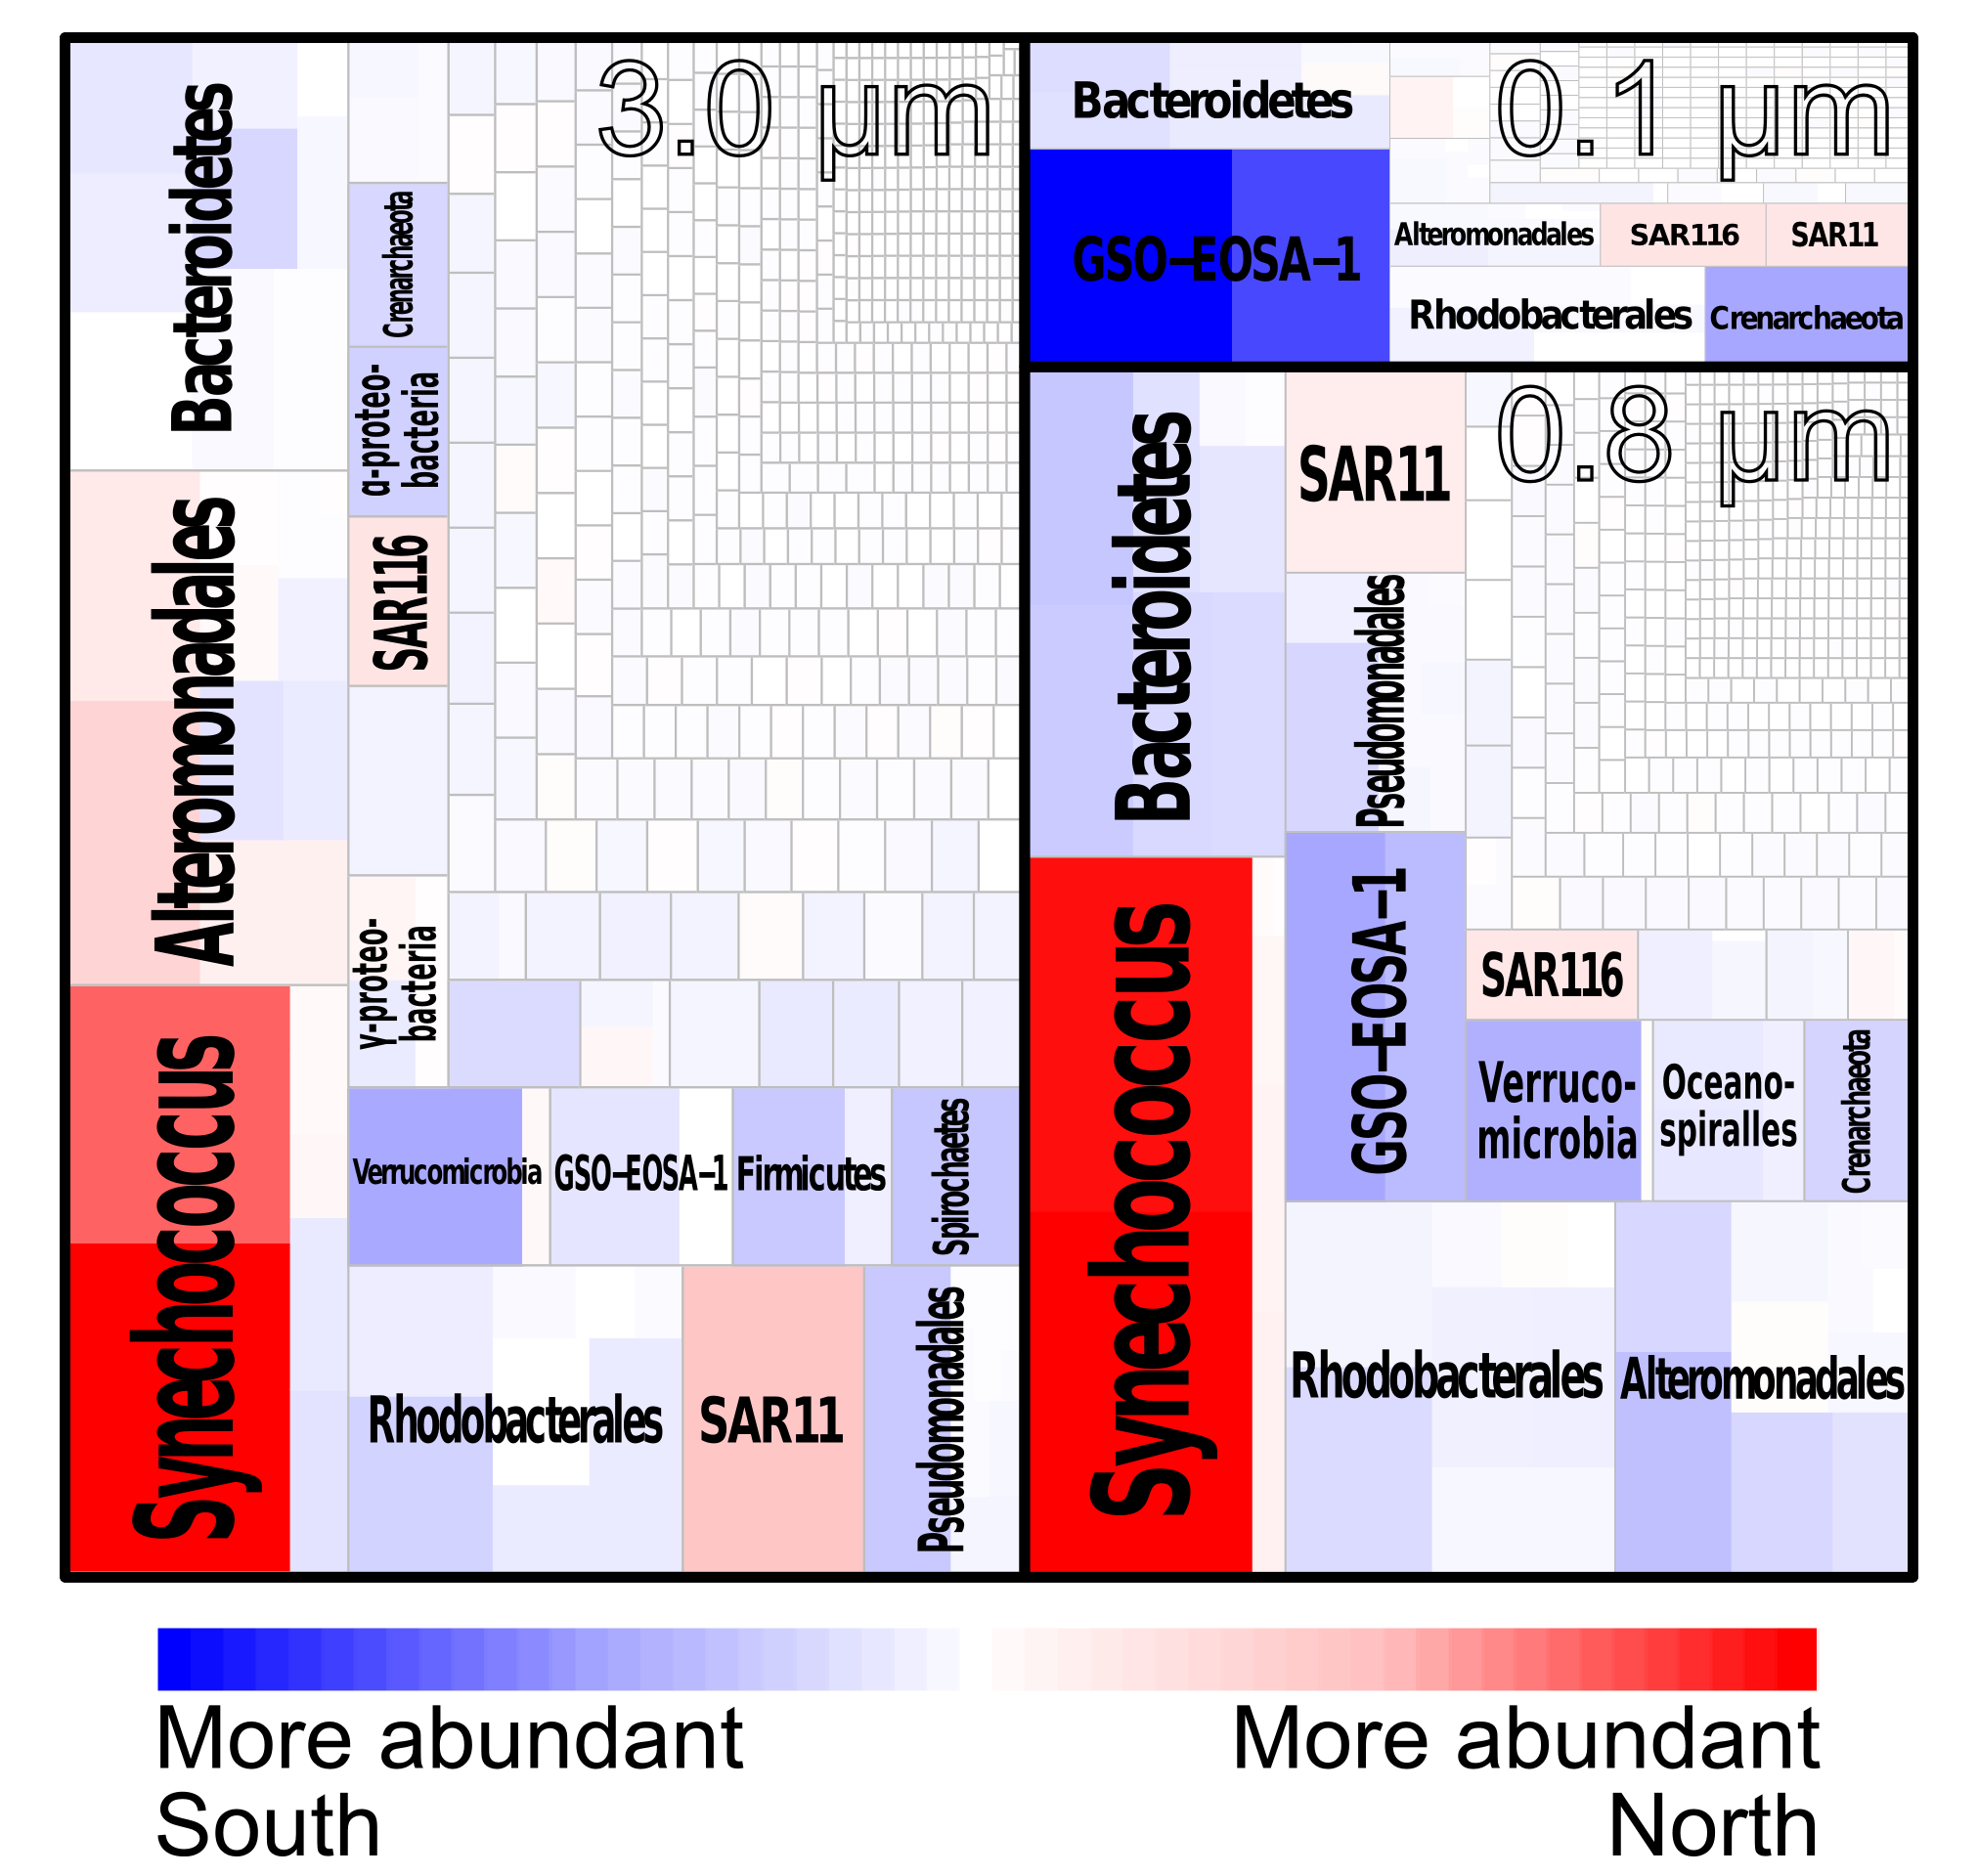
\includegraphics[width=\textwidth]{../polarfront/taxotreemap.png}
  \caption[Contribution of \acp{OTU} to variance between the North and South zones]{Contribution of \acp{OTU} to variance between the North and South zones, and differential abundance of \acp{OTU} from each size fraction between the two zones.
Each coloured (red or blue) rectangle represents an OTU identified through analysis of BLAST matches between SO metagenome data and the RefSeq database.
The area of each rectangle as a proportion of the total plot area corresponds to that \ac{OTU}'s contribution to the total variance between the two zones.
The colour of each rectangle corresponds to difference in relative abundance of that OTU between the zones, with blue indicating a higher relative abundance south of the PF, and red a higher abundance north of the PF.
\acp{OTU} from clades or taxonomic ranks of interest have been grouped, with labels in bold and groups separated by gray lines. 
Groups and \acp{OTU} with a low contribution to variance which were not grouped are unlabeled.
\acp{OTU} from each size fraction have also been grouped, with labels in black outline and size fractions separated by thick black lines. 
The data used to generate this figure are given in the supplementary material \suppfile{PF-OTUs-SIMPER.csv}.
  }
  \label{fig:taxotreemap}
\end{figure}


TODO nMDS

TODO HERE 
\subsubsection{Validation of \softwarename{minspec}}
\subsection{Functional analysis of metagenomic data}

\section{Discussion}

\section{Conclusions}

